\documentclass[12pt]{article}

\usepackage{amsmath, mathtools}
\usepackage{amsfonts}
\usepackage{amssymb}
\usepackage{graphicx}
\usepackage{colortbl}
\usepackage{xr}
\usepackage{hyperref}
\usepackage{longtable}
\usepackage{xfrac}
\usepackage{tabularx}
\usepackage{float}
\usepackage{siunitx}
\usepackage{booktabs}
\usepackage{caption}
\usepackage{pdflscape}
\usepackage{afterpage}

\usepackage[round]{natbib}
%\usepackage{refcheck}

\hypersetup{
    bookmarks=true,         % show bookmarks bar?
    colorlinks=true,       % false: boxed links; true: colored links
    linkcolor=red,          % color of internal links (change box color with linkbordercolor)
    citecolor=green,        % color of links to bibliography
    filecolor=magenta,      % color of file links
    urlcolor=cyan           % color of external links
}

%% Comments

\usepackage{color}

%\newif\ifcomments\commentstrue %displays comments
\newif\ifcomments\commentsfalse %so that comments do not display

\ifcomments
\newcommand{\authornote}[3]{\textcolor{#1}{[#3 ---#2]}}
\newcommand{\todo}[1]{\textcolor{red}{[TODO: #1]}}
\else
\newcommand{\authornote}[3]{}
\newcommand{\todo}[1]{}
\fi

\newcommand{\wss}[1]{\authornote{blue}{SS}{#1}} 
\newcommand{\plt}[1]{\authornote{magenta}{TPLT}{#1}} %For explanation of the template
\newcommand{\an}[1]{\authornote{cyan}{Author}{#1}}

%% Common Parts

\newcommand{\progname}{Mechatronics Engineering} % PUT YOUR PROGRAM NAME HERE
\newcommand{\authname}{Team 25, Preliminary
\\ Ahmed Nazir, nazira1
\\ Stephen Oh, ohs9
\\ Muhanad Sada, sadam
\\ Tioluwalayomi Babayeju, babayejt} % AUTHOR NAMES                  

\usepackage{hyperref}
    \hypersetup{colorlinks=true, linkcolor=blue, citecolor=blue, filecolor=blue,
                urlcolor=blue, unicode=false}
    \urlstyle{same}
                                


% For easy change of table widths
\newcommand{\colZwidth}{1.0\textwidth}
\newcommand{\colAwidth}{0.13\textwidth}
\newcommand{\colBwidth}{0.82\textwidth}
\newcommand{\colCwidth}{0.1\textwidth}
\newcommand{\colDwidth}{0.05\textwidth}
\newcommand{\colEwidth}{0.8\textwidth}
\newcommand{\colFwidth}{0.17\textwidth}
\newcommand{\colGwidth}{0.5\textwidth}
\newcommand{\colHwidth}{0.28\textwidth}

% Used so that cross-references have a meaningful prefix
\newcounter{defnum} %Definition Number
\newcommand{\dthedefnum}{GD\thedefnum}
\newcommand{\dref}[1]{GD\ref{#1}}
\newcounter{datadefnum} %Datadefinition Number
\newcommand{\ddthedatadefnum}{DD\thedatadefnum}
\newcommand{\ddref}[1]{DD\ref{#1}}
\newcounter{theorynum} %Theory Number
\newcommand{\tthetheorynum}{T\thetheorynum}
\newcommand{\tref}[1]{T\ref{#1}}
\newcounter{tablenum} %Table Number
\newcommand{\tbthetablenum}{T\thetablenum}
\newcommand{\tbref}[1]{TB\ref{#1}}
\newcounter{assumpnum} %Assumption Number
\newcommand{\atheassumpnum}{P\theassumpnum}
\newcommand{\aref}[1]{A\ref{#1}}
\newcounter{goalnum} %Goal Number
\newcommand{\gthegoalnum}{P\thegoalnum}
\newcommand{\gsref}[1]{GS\ref{#1}}
\newcounter{instnum} %Instance Number
\newcommand{\itheinstnum}{IM\theinstnum}
\newcommand{\iref}[1]{IM\ref{#1}}
\newcounter{reqnum} %Requirement Number
\newcounter{reqnumDA} %Requirement Number
\newcounter{reqnumDAP} %Requirement Number
\newcommand{\rthereqnum}{P\thereqnum}
\newcommand{\rref}[1]{R\ref{#1}}
\newcounter{nfrnum} %NFR Number
\newcommand{\rthenfrnum}{NFR\thenfrnum}
\newcommand{\nfrref}[1]{NFR\ref{#1}}
\newcounter{lcnum} %Likely change number
\newcounter{ulcnum}
\newcommand{\lthelcnum}{LC\thelcnum}
\newcommand{\lcref}[1]{LC\ref{#1}}

\usepackage{fullpage}


\begin{document}

\title{Software Requirements Specification \progname: Formulate} 

\author{\authname}
\date{\today}
	
\maketitle

~\newpage

\pagenumbering{arabic}

\tableofcontents

~\newpage

\section*{Revision History}

\begin{tabularx}{\textwidth}{p{3cm}p{2cm}X}
\toprule {\bf Date} & {\bf Version} & {\bf Notes}\\
\midrule
Date 1 & 1.0 & Notes\\
Date 2 & 1.1 & Notes\\
\bottomrule
\end{tabularx}

~\newpage

\section{Introduction}

\subsection{Document Purpose}

This document provides the set of Software Requirements Specifications (SRS) used to describe the system developed to assist testing efforts in technical teams. Both hardware and software system requirements were included to fully specify all system requirements. \\

The user can expect to understand the system behavior under expected use cases, the functional and non-functional requirements the system must adhere to, and a phase in development plan.\\

\subsection{Project Description}

Effective test data collection and storage is a common challenge extra-curricular teams face in the technical domain. In teams who do not invest in streamlining data collection and storage, teams cannot fully utilize test data to validate designs. As a result, teams encounter difficulty proving design validity during competition, experience reduced competitiveness when presenting an under-validated system, and fail to generate trends on aggregated test data to efficiently find areas of improvement in design. \\

Project "Formulate" enables Formula teams to streamline data collection and storage, resulting in testing overhead reduction and increased control of raw test data gathered by automating aspects of the testing procedure.\\

\subsection{Project Scope}

Project Formulate aims to provide the McMaster Formula Electric team with a well-documented and complete system. To accomplish the project goals within an 8 month timeline, the following scope of requirements were developed to set clear boundaries on deliverables.\\

\newpage

\noindent
  In of Scope Items:
  \begin{enumerate}
\item Documentation for device integration into testing workflows for common tests
\item Hardware capable of collecting data from test equipment
\item User interface to interact with raw data and submit the data to a database
\item Record of organized, historical data
\item Visualization of test data stored in a database with auto-generated KPI metrics
  \end{enumerate}
  Out of Scope Items:

  \begin{enumerate}
\item Custom website to visualize test data results stored in a database
\item Security through data encryption
\item Predictive intelligence to estimate if rate of test data collected is on track to produce a fully validated product
  \end{enumerate}

\subsection{Table of Symbols}

\renewcommand{\arraystretch}{1.2}
%\noindent \begin{tabularx}{1.0\textwidth}{l l X}
\noindent \begin{longtable*}{l l p{12cm}} \toprule
\textbf{Symbol} & \textbf{Unit} & \textbf{Description}\\
\midrule 
$A_C$ & \si[per-mode=symbol] {\square\metre} & coil surface area\\
\bottomrule
\end{longtable*}


\subsection{Abbreviations and Acronyms}

\renewcommand{\arraystretch}{1.2}
%\noindent \begin{tabular}{l l} 
\noindent \begin{longtable*}{l p{13cm}} 
  \toprule		
  \textbf{Symbol} & \textbf{Description}\\
  \midrule 
  SAE & Society of Automotive Engineers\\
  LC & Likely Change\\
  ULC & Unlikely to Change\\
  SRS & Software Requirements Specification\\
  DBTL & Design Build Test Learning\\
  KPI & Key Performance Indicators\\
  FR & Functional Requirements\\
  NFR & Non-functional Requirements\\
  PC & Personal Computer\\
  CAD & Computer Aided Design\\

  
  \bottomrule
%\end{tabular}\\
\end{longtable*}


\section{User Characteristics}


\subsection{Stakeholders}


\subsection{Use Cases} 

\subsection{User Consideration}

\subsection{Impact}


\section{System Description}

\subsection{Assumptions}

\subsection{Context Diagram}
\begin{figure}[h!]
\begin{center}
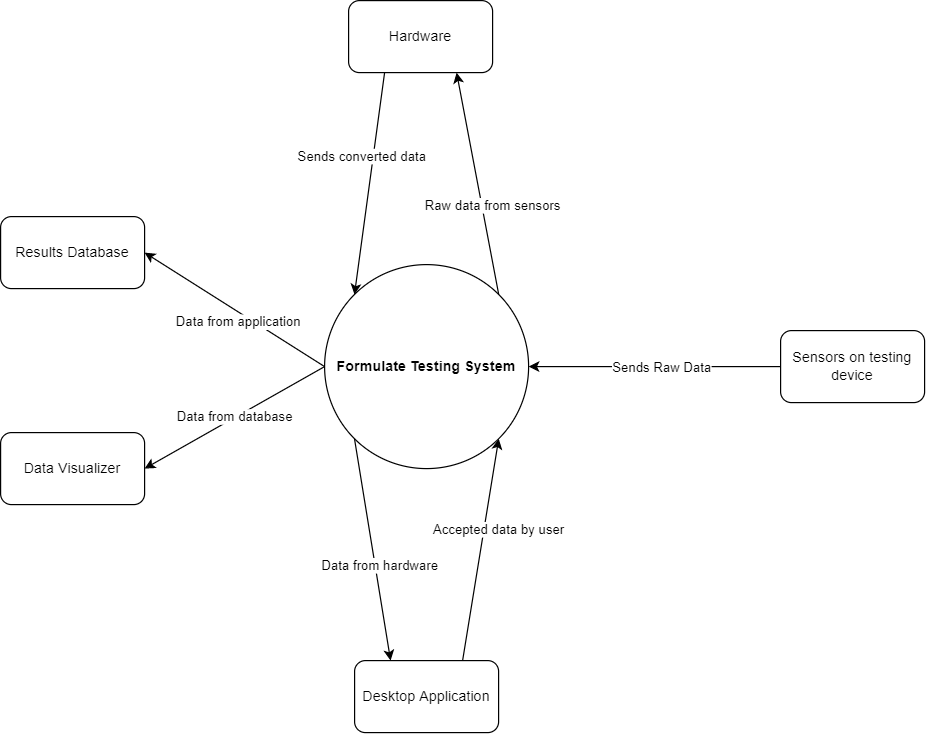
\includegraphics[width=0.9\textwidth]{sys_context_diagram}
\caption{System Context Diagram}
\label{Fig_SystemContext} 
\end{center}
\end{figure}

\subsection{State Transition Diagram}

\subsection{Monitored and Controlled Variables}
  \begin{tabular}{| p{0.23\textwidth} | p{0.10\textwidth}| p{0.10\textwidth}| p{0.46\textwidth}|}
    \hline
    \rowcolor[gray]{0.9}
    Monitored Variable & Type & Units & Description\\
    \hline
    m\_vibration & Analog& V& A signal monitoring the vibration resistance of the motor \\
    \hline
    m\_humidity & Analog & V & A signal monitoring the humidity of the motor’s environment \\
    \hline
    m\_temperature & Analog & V & A signal monitoring the temperature of the motor’s environment \\
    \hline
    m\_shock & Analog & V & A signal monitoring the shock resistance of the motor \\
    \hline
    m\_conv\_vibration & Digital & g  & Converted vibration values that are in useful units \\
    \hline
    m\_conv\_humidity & Digital & \% & Converted humidity values that are in useful units \\
    \hline
    m\_conv\_temperature & Digital & \textdegree C & Converted temperature values that are in useful units \\
    \hline
    m\_conv\_shock & Digital & g & Converted shock values that are in useful units \\
    \hline
    m\_data\_accepted & Digital & T/F & Determines if user has accepted the results and wants to send it to the database \\
    \hline
  \end{tabular}
%\\Table 1.0: Monitored Variables
\\ \\ \\
\begin{tabular}{| p{0.23\textwidth} | p{0.10\textwidth}| p{0.10\textwidth}| p{0.46\textwidth}|}
    \hline
    \rowcolor[gray]{0.9}
    Controlled Variable & Type & Units & Description\\
    \hline
    c\_green\_light& Digital& 1/0& Green LED light on testing device that indicates passed measurements \\
    \hline
    c\_red\_light& Digital & 1/0 & Red LED light on testing device that indicates failed measurements \\
    \hline
    c\_sent\_to\_database & Digital & T/F & Determines if results displayed on the application are sent to the database \\
    \hline
  \end{tabular}
  %\\Table 2.0: Controlled Variables
  \\ \\ \\
  \begin{tabular}{| p{0.23\textwidth} | p{0.10\textwidth}| p{0.10\textwidth}| p{0.46\textwidth}|}
    \hline
    \rowcolor[gray]{0.9}
    Constant & Units & Value & Description\\
    \hline
    k\_temperature\_range& \textdegree C& 5-40& Acceptable ambient temperature values for a Formula Electric motor \\
    \hline
    k\_humidity\_range& \% & 5-85 & Acceptable relative humidity values for a Formula electric motor \\
    \hline
    k\_max\_shock & g & 100 & Maximum shock resistance for a Formula Electric motor \\
    \hline
    k\_max\_vibration & g & 20 & Maximum vibration resistance for a Formula Electric motor \\
    \hline
  \end{tabular}
%  \\Table 3.0: Controlled Variables
\\
\subsection{Functional Decomposition Diagram}
\begin{figure}[h!]
  \begin{center}
  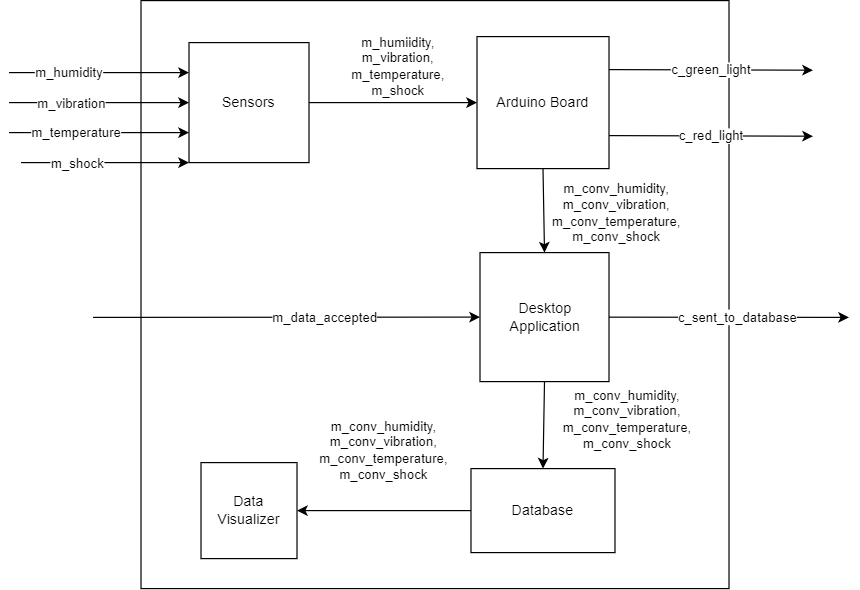
\includegraphics[width=0.9\textwidth]{functional_decomposition}
  \caption{Functional Decomposition Diagram}
  \label{Fig_FunctionalDecomposition} 
  \end{center}
  \end{figure}

\section{Requirements}

\subsection{Functional Requirements}
Formulate consists of 3 main components, each with its own functional requirements. The device addresses the sensors and physical device which interacts directly with the user. The desktop application is the means for the user to select modes and submit data, and the data analytics platform (website) is for the user to view old test case data to check if KPI's are met.

\subsubsection{Priority 1} 

\begin{itemize}
  
  \item[FR \refstepcounter{reqnum}\thereqnum:] The device should be able to measure vibration, temperature, humidity, and shock
  
  \item[FR \refstepcounter{reqnum}\thereqnum:] The device should connect to a PC wired to transmit data
  
  \item[FR \refstepcounter{reqnum}\thereqnum:] The device should have a start button which activates the telemetry to start reading values between the PC and device 
  
  \item[FR \refstepcounter{reqnum}\thereqnum:] The device should have a stop button which stops the telemetry stops reading values between the PC and device
  
  \item[FR \refstepcounter{reqnum}\thereqnum:] The application should allow users to preview the data after a test

  \item[FR \refstepcounter{reqnum}\thereqnum:] The application should allow the user to send the data to the database
  
  \item[FR \refstepcounter{reqnum}\thereqnum:] The website should be able to read the data from the database
  
  \end{itemize}


\subsubsection{Priority 2}
\begin{itemize}

  \item[FR \refstepcounter{reqnum}\thereqnum:] The device should easily mount to the Formula SAE car

  \item[FR \refstepcounter{reqnum}\thereqnum:] The device should contain a rechargeable battery
  \begin{description} \item[Rationale:] The device needs its own independent power source which will allow for it to be placed in areas without a power socket. \end{description}

  \item[FR \refstepcounter{reqnum}\thereqnum:] The device should connect to a PC wirelessly to transmit data

  \item[FR \refstepcounter{reqnum}\thereqnum:] The device should have a screen to display the current status to the user
  
  \item[FR \refstepcounter{reqnum}\thereqnum:] The modular sensors should have a snap on mounting mechanism to connect to the base
  \begin{description} \item[Rationale] Modular sensors need to have a rigid connection with the board with minimal movement to get the most accurate values from the sensor  \end{description}

  \item[FR \refstepcounter{reqnum}\thereqnum:] The application should show live raw data from the sensors
  
  \item[FR \refstepcounter{reqnum}\thereqnum:] The application should allow the user to trim the data before sending it to the database
  
  \item[FR \refstepcounter{reqnum}\thereqnum:] The application should allow the user to configure the device's settings
  \begin{description} \item[Rationale:] The device will need to have the wifi setting configured which will be done in the application \end{description}
  
  \end{itemize}

\subsubsection{Priority 3}
\begin{itemize}
  \item[FR \refstepcounter{reqnum}\thereqnum:] The device should have 4 connection ports to add module sensors to it
  \begin{description} \item[Rationale] Each connection port will make the device more modular and allow for users to add more sensors in the future for other tests.  \end{description}

  \item[FR \refstepcounter{reqnum}\thereqnum:] The website should only allow users who have access to view the data
  
  \item[FR \refstepcounter{reqnum}\thereqnum:] The website should have the option to filter out the data by test conducted
  
  \item[FR \refstepcounter{reqnum}\thereqnum:] The website should show whether the tests passed according to threshold values
  
  \item[FR \refstepcounter{reqnum}\thereqnum:] The application should allow the user to trim the data before sending it to the database
  
  \item[FR \refstepcounter{reqnum}\thereqnum:] Any data pushed to the database should not be editable by the user
  
  \item[FR \refstepcounter{reqnum}\thereqnum:] The device should alert the user if any tests exceed the operating condition of the car
  \begin{description} \item[Rationale] If at any point during the test it exceed operating conditions, the devices should make it obvious to the user  \end{description}
  
  \end{itemize}

\newpage
\subsection{Nonfunctional Requirements}

\noindent\begin{itemize}

\subsubsection{Usability} 

    \item[NFR\refstepcounter{nfrnum}\thenfrnum:]
    \textbf{Ease of Learning}\\
    The user will be able to learn the device's operation quickly to integrate into their testing workflow efficiently\\

    \item[NFR\refstepcounter{nfrnum}\thenfrnum:]
    \textbf{Ease of Use}\\
    The system will be fast at processing data such that additional overhead through the use of the device is less than if all components of the testing workflow were completed individually.\\

\subsubsection{Performance} 

    \item[NFR\refstepcounter{nfrnum}\thenfrnum:]
    \textbf{Speed}\\
    The system bandwidth will be high enough to support testing equipment with high data collection frequencies.\\

    \item[NFR\refstepcounter{nfrnum}\thenfrnum:]
    \textbf{Reliability and Availability}\\
    The system will be fail-safe to withstand single point of failures in components with high probability of operational failure.\\

\subsubsection{Operational}

    \item[NFR\refstepcounter{nfrnum}\thenfrnum:]
      \textbf{Expected Technological Environment}\\
    The device will be able to facilitate a variety of tests using a range of equipment, as long as the equipment is compatible with the data measuring hardware.\\

    \item[NFR\refstepcounter{nfrnum}\thenfrnum:]
    \textbf{Expected Physical Environment}
    The system will be operational under a wide range of temperatures and operational vibrations.\\

\subsubsection{Maintainability and Portability}

    \item[NFR\refstepcounter{nfrnum}\thenfrnum:]
      \textbf{Maintainability}\\
    The system will be modular and have low cohesion such that users can adapt elements of the device's hardware and software infrastructure to current needs without breaking other elements.\\

    \item[NFR\refstepcounter{nfrnum}\thenfrnum:]
    \textbf{Portability}\\
    The user's ability to conduct tests will not be affected by the physical constraints from the device.\\
  
\subsubsection{Security}

    \item[NFR\refstepcounter{nfrnum}\thenfrnum:]
    \textbf{Software Integrity}\\
    The system will be secure against malicious spam aimed at reducing validity of aggregate test data stored in the database.\\

\subsubsection{Cultural and Political}

    N/A\\

\subsubsection{Legal}

    N/A\\zzz

\end{itemize}


\subsection{Likely Changes}    

\noindent \begin{itemize}

\item[LC\refstepcounter{lcnum}\thelcnum\label{LC_meaningfulLabel}:] Starting and stopping the device to get data using hardware
\begin{description} \item[Rationale:] When the device is connected to the computer we can remote start and stop it using software \end{description}

\item[LC\refstepcounter{lcnum}\thelcnum\label{LC_meaningfulLabel}:] The base data we are collecting (Vibration, Shock, Temperature, Humidity)
\begin{description} \item[Rationale:] Since the device is set to be modular we might change those initial values we are testing with other ones \end{description}

\item[LC\refstepcounter{lcnum}\thelcnum\label{LC_meaningfulLabel}:] The number of modular ports on the base device
\begin{description} \item[Rationale:] When the device is connected to the computer we can remote start and stop it using software \end{description}


\end{itemize}

\subsection{Unlikely Changes}    

\noindent \begin{itemize}

\item[ULC\refstepcounter{ulcnum}\theulcnum:] The sensors will remain modular to adapt to different tests that need to be conducted
\begin{description} \item[Rationale:] The product should be expandable in the future to be able to test different values \end{description}

\end{itemize}

\section{Development Plan}

The development plan is categorized into multiple sections, where each section represented a significant phase in the progress of project execution. A section is given a number in the hundreds (X00) to denote a significant phase in the project. Each section is subdivided further into segments given by numbers specified in the tens (XX0) to denote smaller steps within each phase. The expected order of segment completion follows the order of increasing number count; the lowest number segment should be completed first and the highest number segment should be completed last.\\

Each segment has an overall goal that can include the coordination of multiple teammates. Upon completion of each segment, the team members relevant to the segment review and buyoff the readyness of the segment. Upon completion of buying off each segment within a section, the overall phase is considered to be bought off and completed with confidence. The relevant stakeholders must aim to buyoff each segment in a phase before the phase deadline.\\


\noindent
Phase 0: Preperation (000 series)\\
Phase 0 Deadline: October 28, 2022\\

\begin{table}[H]
  \centering
  \begin{tabular}{|p{2cm}|p{10cm}|p{2cm}|}
  \hline
  \multicolumn{1}{|c|}{\textbf{000 Buyoffs}} & \multicolumn{1}{c|}{\textbf{Explanation}} & \multicolumn{1}{|c|}{\textbf{Stakeholder(s)}}
  \\ \hline
  010
  & Purchase sensor equipment, data measurement hardware, 3D print material.
  & Stephen
  \newline                                
  \\ \hline

  020                              
  & Obtain licenses for 3D CAD software use and database access
  & Stephen
  \newline                                
  \\ \hline

  030                          
  & Document material costs and licensing constraints
  & Stephen
  \newline                                
  \\ \hline

  040                                
  & Distribute materials and licensing to relevant project area Stakeholder
  & Stephen 
  \newline                            
  \\ \hline

  050                                
  & Completion of device chassis mechanical design and modelling
  & Stephen 
  \newline                            
  \\ \hline

  060                                
  & Completion of electrical connection hardware circuit design and schematic
  & Stephen 
  \newline                            
  \\ \hline

  090                                
  & Device chassis manufactured
  & Stephen 
  \newline                            
  \\ \hline

  \end{tabular}
\end{table}
\newpage

\noindent
Phase 1: Proof of Concept (100 series)\\
Phase 1 Deadline: November 11, 2022\\
\begin{table}[H]
  \centering
  \begin{tabular}{|p{2cm}|p{10cm}|p{2cm}|}
  \hline
  \multicolumn{1}{|c|}{\textbf{100 Buyoffs}} & \multicolumn{1}{c|}{\textbf{Explanation}} & \multicolumn{1}{|c|}{\textbf{Stakeholder(s)}}
  \\ \hline
  110
  & Desktop application program developed with basic user interface
  & Stephen
  \newline                                
  
  \\ \hline
  120                              
  & Desktop application program can recieve data from data measurement device using a wired connection
  & Stephen
  \newline                                

  \\ \hline
  130                          
  & Desktop application program can interface with database to send data
  & Stephen
  \newline                                

  \\ \hline
  140                                
  & Desktop application program can edit data from data measurement device before sending it to the database
  & Stephen 
  \newline                            

    \\ \hline
  150                                
  & Visualization application can pull data and generate KPI metrics from the database
  & Stephen 
  \newline 

  \\ \hline
  160                                
  & Integration between data measurement device and desktop application
  & Stephen 
  \newline 

  \\ \hline
  170                                
  & Integration between desktop application and visualization application
  & Stephen 
  \newline 

  \\ \hline
  190                                
  & Integration between data measurement device, desktop application, and data measurement device
  & Stephen 
  \newline 
  \\ \hline


  \end{tabular}
\end{table}

\newpage
\noindent
Phase 2: Revision 0 Presentation (200 series)\\
Phase 2 Deadline: February 3, 2023\\

\begin{table}[H]
  \centering
  \begin{tabular}{|p{2cm}|p{10cm}|p{2cm}|}
  \hline
  \multicolumn{1}{|c|}{\textbf{200 Buyoffs}} & \multicolumn{1}{c|}{\textbf{Explanation}} & \multicolumn{1}{|c|}{\textbf{Stakeholder(s)}}
  \\ \hline
  210
  & Mechanical design and modelling completion of physical user interface components on device chassis and connection modules
  & Stephen
  \newline                                
  \\ \hline

  220                              
  & Completion of wireless communication between data measurement device and desktop application 
  & Stephen
  \newline                                
  \\ \hline

  230                          
  & Completion of database security against tests that break utility of database
  & Stephen
  \newline                                
  \\ \hline

  290                                
  & Completion of extended KPI features for visualization application
  & Stephen 
  \newline                            
  \\ \hline

  \end{tabular}
\end{table}
\newpage

\noindent
Phase 3: Final Demonstrations (300 series)\\
Phase 3 Deadline: March 17, 2023\\






\newpage

\bibliographystyle {plainnat}
\bibliography {../../refs/References}

\newpage

\noindent \plt{The following is not part of the template, just some things to consider
  when filing in the template.}

\noindent \plt{Grammar, flow and \LaTeX advice:
\begin{itemize}
\item For Mac users \texttt{*.DS\_Store} should be in \texttt{.gitignore}
\item \LaTeX{} and formatting rules
\begin{itemize}
\item Variables are italic, everything else not, includes subscripts (link to
  document)
\begin{itemize}
\item \href{https://physics.nist.gov/cuu/pdf/typefaces.pdf}{Conventions}
\item Watch out for implied multiplication
\end{itemize}
\item Use BibTeX
\item Use cross-referencing
\end{itemize}
\item Grammar and writing rules
\begin{itemize}
\item Acronyms expanded on first usage (not just in table of acronyms)
\item ``In order to'' should be ``to''
\end{itemize}
\end{itemize}}

\noindent \plt{Advice on using the template:
\begin{itemize}
\item Difference between physical and software constraints
\item Properties of a correct solution means \emph{additional} properties, not
  a restating of the requirements (may be ``not applicable'' for your problem).
  If you have a table of output constraints, then these are properties of a
  correct solution.
\item Assumptions have to be invoked somewhere
\item ``Referenced by'' implies that there is an explicit reference
\item Think of traceability matrix, list of assumption invocations and list of
  reference by fields as automatically generatable
\item If you say the format of the output (plot, table etc), then your
  requirement could be more abstract
\end{itemize}
}

\end{document}